%----------------------------------------------------------------------------------------
%    PACKAGES AND THEMES
%----------------------------------------------------------------------------------------

\documentclass[aspectratio=169,xcolor=dvipsnames]{beamer}
\usetheme{SimpleDarkBlue}

\usepackage{hyperref}
\usepackage{graphicx} % Allows including images
\usepackage{booktabs} % Allows the use of \toprule, \midrule and \bottomrule in tables

%----------------------------------------------------------------------------------------
%    TITLE PAGE
%----------------------------------------------------------------------------------------

\title{Human-Benchmark}
\subtitle{2 Laboratorinis}

\author{Adrian, Arnas, Darius, Tadas}

\institute
{
    Matematikos ir informatikos fakultetas \\
    Vilniaus universitetas % Your institution for the title page
}
% \date{\today} % Date, can be changed to a custom date 

%----------------------------------------------------------------------------------------
%    PRESENTATION SLIDES
%----------------------------------------------------------------------------------------

\begin{document}

\begin{frame}
    % Print the title page as the first slide
    \titlepage
\end{frame}

\begin{frame}{Apžvalga}
    % Throughout your presentation, if you choose to use \section{} and \subsection{} commands, these will automatically be printed on this slide as an overview of your presentation
    \tableofcontents
\end{frame}


\section{Robustness diagrams}

\begin{frame}{Core Functionality (Robustness diagram)}
    \begin{figure}[H]
        \centering
        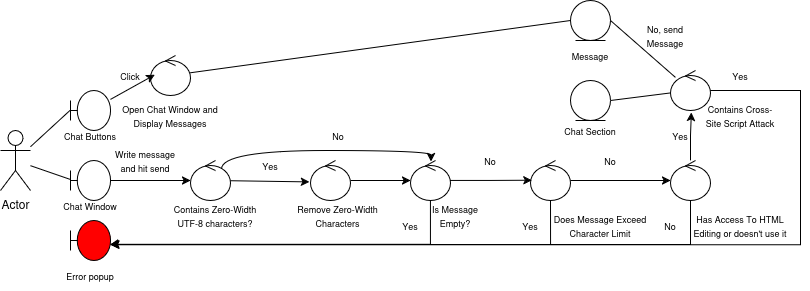
\includegraphics[width=0.6\textwidth]{images/Robustness/R Core ChatF.drawio.png}
        \caption{Core Functionality of The Chat}
        \label{fig:appdb}
    \end{figure}
\end{frame}

\begin{frame}{Message Management (Robustness diagram)}
    \begin{figure}[H]
        \centering
        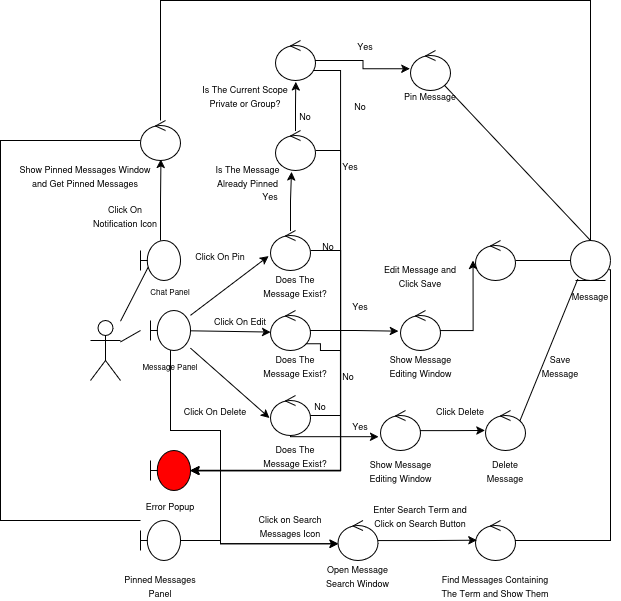
\includegraphics[width=0.6\textwidth]{images/Robustness/R Message ManagementF.drawio.png}
        \caption{Message Managment Capabilities of The Chat}
        \label{fig:appdb}
    \end{figure}
\end{frame}

\begin{frame}{Chat Management (Robustness diagram)}
    \begin{figure}[H]
        \centering
        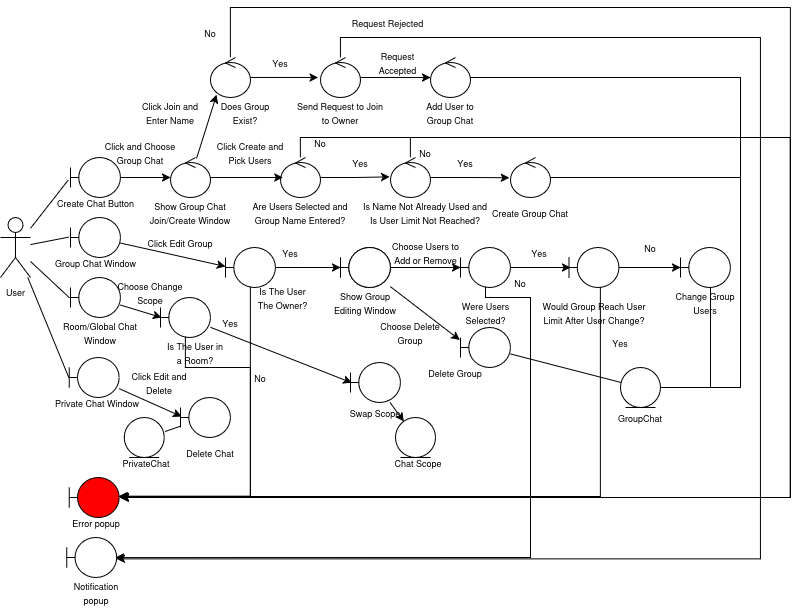
\includegraphics[width=0.6\textwidth]{images/Robustness/R_Chat_managmentF.drawio.png}
        \caption{Chat Managment Capabilities of The Chat}
        \label{fig:appdb}
    \end{figure}
\end{frame}

\begin{frame}{UI Interactions (Robustness diagram)}
    \begin{figure}[H]
        \centering
        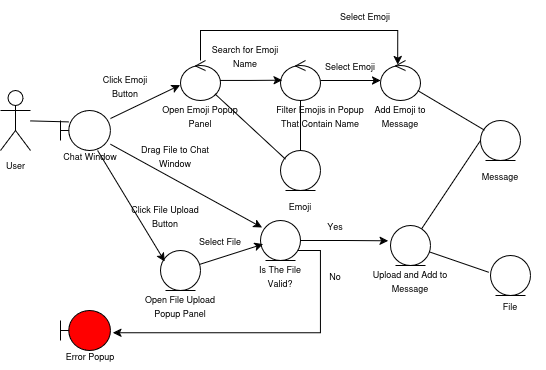
\includegraphics[width=0.6\textwidth]{images/Robustness/R_UI_Interactions.drawio.png}
        \caption{Interactions and Proccesses of The Chat's UI}
        \label{fig:appdb}
    \end{figure}
\end{frame}

\begin{frame}{Administration (Robustness diagram)}
    \begin{figure}[H]
        \centering
        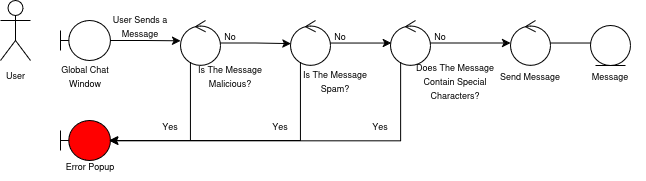
\includegraphics[width=0.6\textwidth]{images/Robustness/R_Administration.drawio.png}
        \caption{Administration Options of The Chat}
        \label{fig:appdb}
    \end{figure}
\end{frame}





%------------------------------------------------


%----------------------------------------------------------------------------------------

\end{document}
